\chapter{Literature Review of Fault Localization in Computer Networks Using
End-to-End Measurements}

This chapter briefly describes three projects (Argus, NetNorad and CEM)
that deploy end-to-end measurements to localize faults in computer networks.

\section{Argus}

In
~\cite{argus_end_to_end_service_anomaly_detection_and_localization_from_an_isps_point_of_view}
is presented Argus, a system to
detect and localize QoS issues in ISP's networks. To achieve this goal, it uses
end-to-end data and network global information, such as
traffic passively monitored at end-users, the ISP network topology,
routing tables, and geographic information. Argus's infrastructure is defined by
the pipeline presented in figure ~\ref{fig:argus_pipeline}.

\begin{figure}[H]
    \centering
    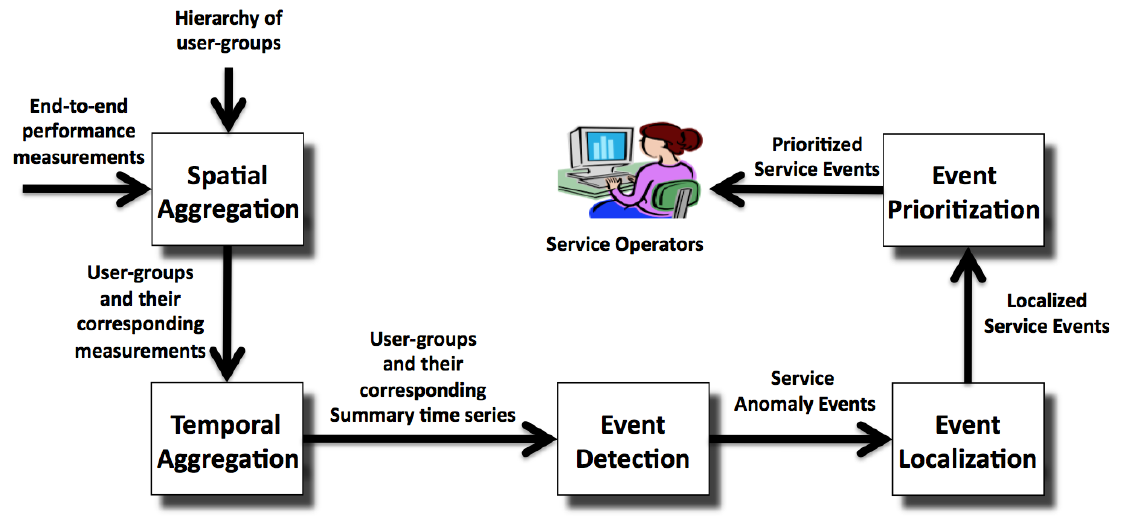
\includegraphics[width=1.0\textwidth]{./figures/literature_review/argus_pipeline.png}
    \caption{Argus pipeline.}
    \label{fig:argus_pipeline}
\end{figure}%

The system operation starts with the spatial aggregation procedure, in which
end-users are clustered into user-groups. This step avoids keeping
track of the end-to-end performance metrics associated with millions of
individual end-users, which improves the system's scalability.
Each user-group is characterized by a set of end-users that share some common
attributes, such as BGP prefix or AS. The used attributes imposes the possible
fault locations to be infered.
An example of an agreggation is presented in figure
~\ref{fig:argus_spatial_aggregation}.

\begin{figure}[H]
    \centering
    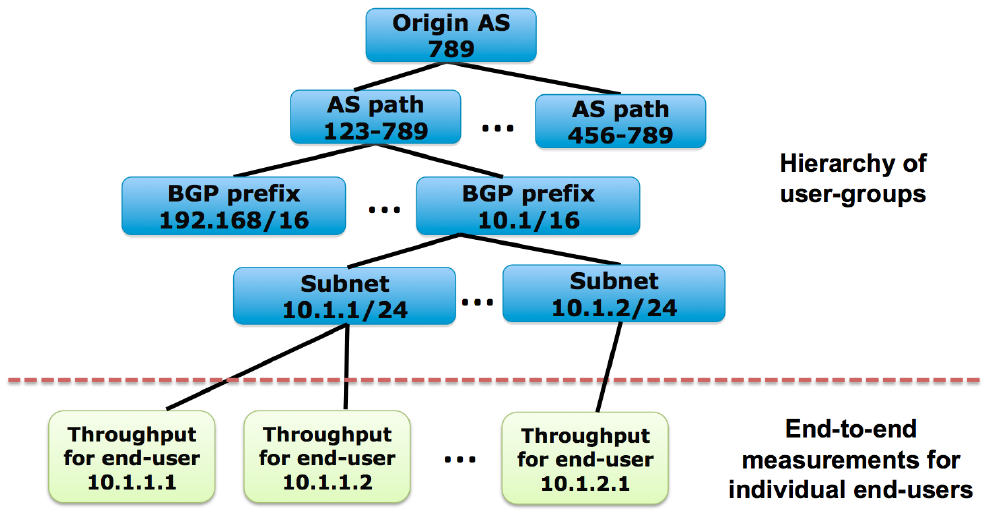
\includegraphics[width=1.0\textwidth]{./figures/literature_review/argus_spatial_aggregation.png}
    \caption{Argus spatial aggregation.}
    \label{fig:argus_spatial_aggregation}
\end{figure}%

The temporal aggregation phase determine how the performance metrics collected
from different end-users in a end-group are aggregated. In this procedure
details about individual end-users are lost, but the goal is to detect events
that impact the user-groups. Instead of analysing the raw individual end-to-end
metrics, Argus focus in summary statistics, such as, percentiles, min, max, of
the distribution, and this can reduce the noisy from raw data, since a
end-group have data from different end-users. For each user-group the
measurements of all end-users are aggregated by time-bins, and for each
time-bin a summary statistics is selected, forming then a summary time series.
Different statistics provides different advantages to track cerain type of
issues, for exaple the min statistics applied to RTT can capture the physical
propagation delay while the average can capture network congestion. Argus uses
median as the default summary statistics, since it was found that empirically,
is effective in tracking service or network issues while being robust to
variability to individual end-users due to their local architecture.

The event detection procedure applies algorithms to detect anomalies in the
summary time series. Argus uses a Holt-Winters variation which is an online
procedure with low runtime and memory complexities, which is essential to the
scale of the system.

Through spatial and anomaly event time correlations Argus is able to localize
fault locations in the network in the event localization procedure, however the
detailed procedure of how this
process is defines was not published.

After the problem localizations the events are sorted according with their
significance, which is defined by a metric obtained through the event detection
algorithm, and considering the number of end-users affected by the event.

Argus was applied to RTT measurements in a CDN hosted in a tier-1 ISP. During a
one month period using time-bins of 1 hour, Argus detected 2909
anomaly events, and in general, lower level user-groups were more responsible
for these anomalies than the higher level groups. For each type of user-group,
only a small fraction of the end-users are responsible for the anomaly events
and the majority of the
anomalies are very short in duration, in which 90\% of the anomilies last for
ar most 1 hour, which was the used time-bin granularity.

The following inferences are not presented in the paper. The fact that only a
small number of end-users are responsible by the anomaly in the summary time
series indicates that fault isolation could achieve higher precision using the
spatial aggregation with finer granularity. It is not clear G-RCA accuracy,
then I don't know if was made a Argus evaluation accuracy. Since the fault
localization  procedure is not presented, it is not possible to check which
topologies types can be used.

\section{NetNorad}

NetNorad ~\cite{netnorad} consists of a Facebook's internal project to
automate the detecion and mitigation of network faults in the Facebook's
network. It is claimed that a human-driven investigation may take minutes or
hours. Also more traditional used network monitoring techiques such as querying
device information through SNMP or via command line interface can not encounter
cases known as gray failures, in which the devices can not properly report its
own malfunctioning. "Or the problem can be associated with the network
structure"

NetNorad is mainly based in end-to-end measurements.
Facebook's servers ping each other, in which
a pinger sends UDP packets to responders, and the latter receive, timestamp
and send the packet back. The process happens in turns, in which each pinger
sends packets to all of its targets, collects the responses, and then repeats
the procedure.

Facebook's network is structured hierarchically. At the
lowest level there are servers in hacks, which are organized in
clusters. A collection of clusters in the same building and serviced by
a common network form a data center. The data centers are aggregated
via a network that interconnects them within the same region and attaches to th
e Facebook global backbone network. This infrastructre spreads across multiple
regions around the world. Figure ~/ref{} presents an example of this
architecture.

ADD IMAGE WITH THE TOPOLOGY

A small number of pingers is deployed in each cluster, but reponders are placed
on
all machines. All pingers share a single global target list, which consists of
at least two machines in every rack.
As with Argus, the system applies aggregation techiques, however, the imposed
hierarchical structure of Facebook can simplify the procedure
. When a pinger receives the responses in a given round, it
aggregates results for machines that belong to the same cluster and tags them
based on their location. Tags are based in the following rules:
"DC" if the target cluster is in the same data center of the pinger,
"Region" if the target cluster is outside the
data center but within the same region, "Global" if it is outside the pinger's
region.

Each cluster have three time series reflecting different
viewpoints, one for the same data center, other for the same region, and other
for the global network. For each time series the system tracks percentiles
over 10-minute
intervals. Tracking multiple percentiles allows the identification of the
nature of the events in the network. For example, a packet loss spike at the
50th percentile means that there is likely a failure affecting the majority of
traffic into or out of a cluster, while a peak at the 90th and not at 50th
percentile would indicate that there is a high level of loss affecting a small
number of targets. For each percentile and proximity tag is defined two
thresholds, one for trigger an alarm and other for clear an alarm. This
infrastructure allows alarms to be raised about 30 seconds far from the event.

Metrics are collected from an end-to-end perspective, therefore it
is necessary to distinguish if the events are caused by an end-host failure or
a network fault. The pinger applies an outlier detection,
discarding targets that reports too high packet loss relative to their general
population. Also the same logic is applied to discard reports from pingers that
have anomalous pattern according to their population.

To localize the fault the following
correlation analysis is applied. If loss to a cluster is reported at data center,
region and global tags, then the fault is probably located at the cluster data center.
If all clusters within a data center report packet loss, then the issue is
likely to be a layer above the clusters. These rules doens't determine the
exact fault location, however a Facebook tool called fbtrcrt, similar to the
UNIX traceroute tool, improves this analysis. fbtracert explores multiple
paths between two endpoints, and can analyse the
packet loss at every hop, correlating the resulting path data to find the
common failure point. When fbtracrt is unable to find the failure, then there
is a human involvemnt to find it.

The following inferences are not presented in the paper. The work doesn't
presents an accuracy analysis.

\section{CEM}

In ~/cite{} is proposed a
framework called Crowdsourcing Event Monitoring (CEM), which aims to realize
online detection (within seconds or minutes), of service-level events through
monitoring software that runs inside or alongside applications on the end
systems where they are used.

In the framework, each end-host uses its own passively gathered
performance information to detect local problems as potential network events
. The framework doesn't care how these events are detected,
as long they
correspond to service-level problems. Concurrent events ocurring in multiple
performance metrics of a service (e.g., download and upload rates), increases the
confidence that the problem is independent of the service. After detecting the
events a end-host pushes them to a distributed storage to further analysis. The
fact that the events detection procedures are realized at the end-hosts
increases the scability of the system.

To isolate
the scope of the network events, multiple locally detected events are
correlated from the same network region. This correlation is made in a central
fashion.
The first problem to tacked is to reason if concurrent events are caused by a
network fault. There are several reasons to different hosts experiences
concurrent events. One is the target of the work, which is a network fault.
Another one is that the service can experience a problem not caused by the
network, for example, a high volume of requests in a web service. Also it is
possible that concurrent events occur only by chance, for example, users
experience interference on separate wireless routers. To solve this problem the
framework provides a statistical model to determine if
concurrently events are a coincidence or not. This model takes in
consideration service-specific dependencies and the rate of observed local
events ocurring at the same the same time in a network. In this model, the
confidence in a detected event being due to a network increases with the
number of hosts detecting the event, and with the increase of independent
performance metrics indicating the event. To isolate the problem the framework
uses structure information about the network and the hosts geographic
locations, however, ther work doesn't provides any details of how this
correlation is made.

CEM was deployed and evaluated in a P2P system, using BitTorrent traces collected
from users of the Ono plugin for the Vuze BitTorrent client. The detected
events by the system was compared to aground truth
of network events gathered from public available event reports of ISPs.

The following inferences are not presented in the paper.
CEM provides a high level framework structure, however lack for several details
in the deployment procedure.
